\documentclass{standalone}
\usepackage{tikz}
\usetikzlibrary{patterns, positioning}
\usepackage[sfdefault]{ClearSans} %% option 'sfdefault' activates Clear Sans as the default text font
\usepackage[T1]{fontenc}

\begin{document}
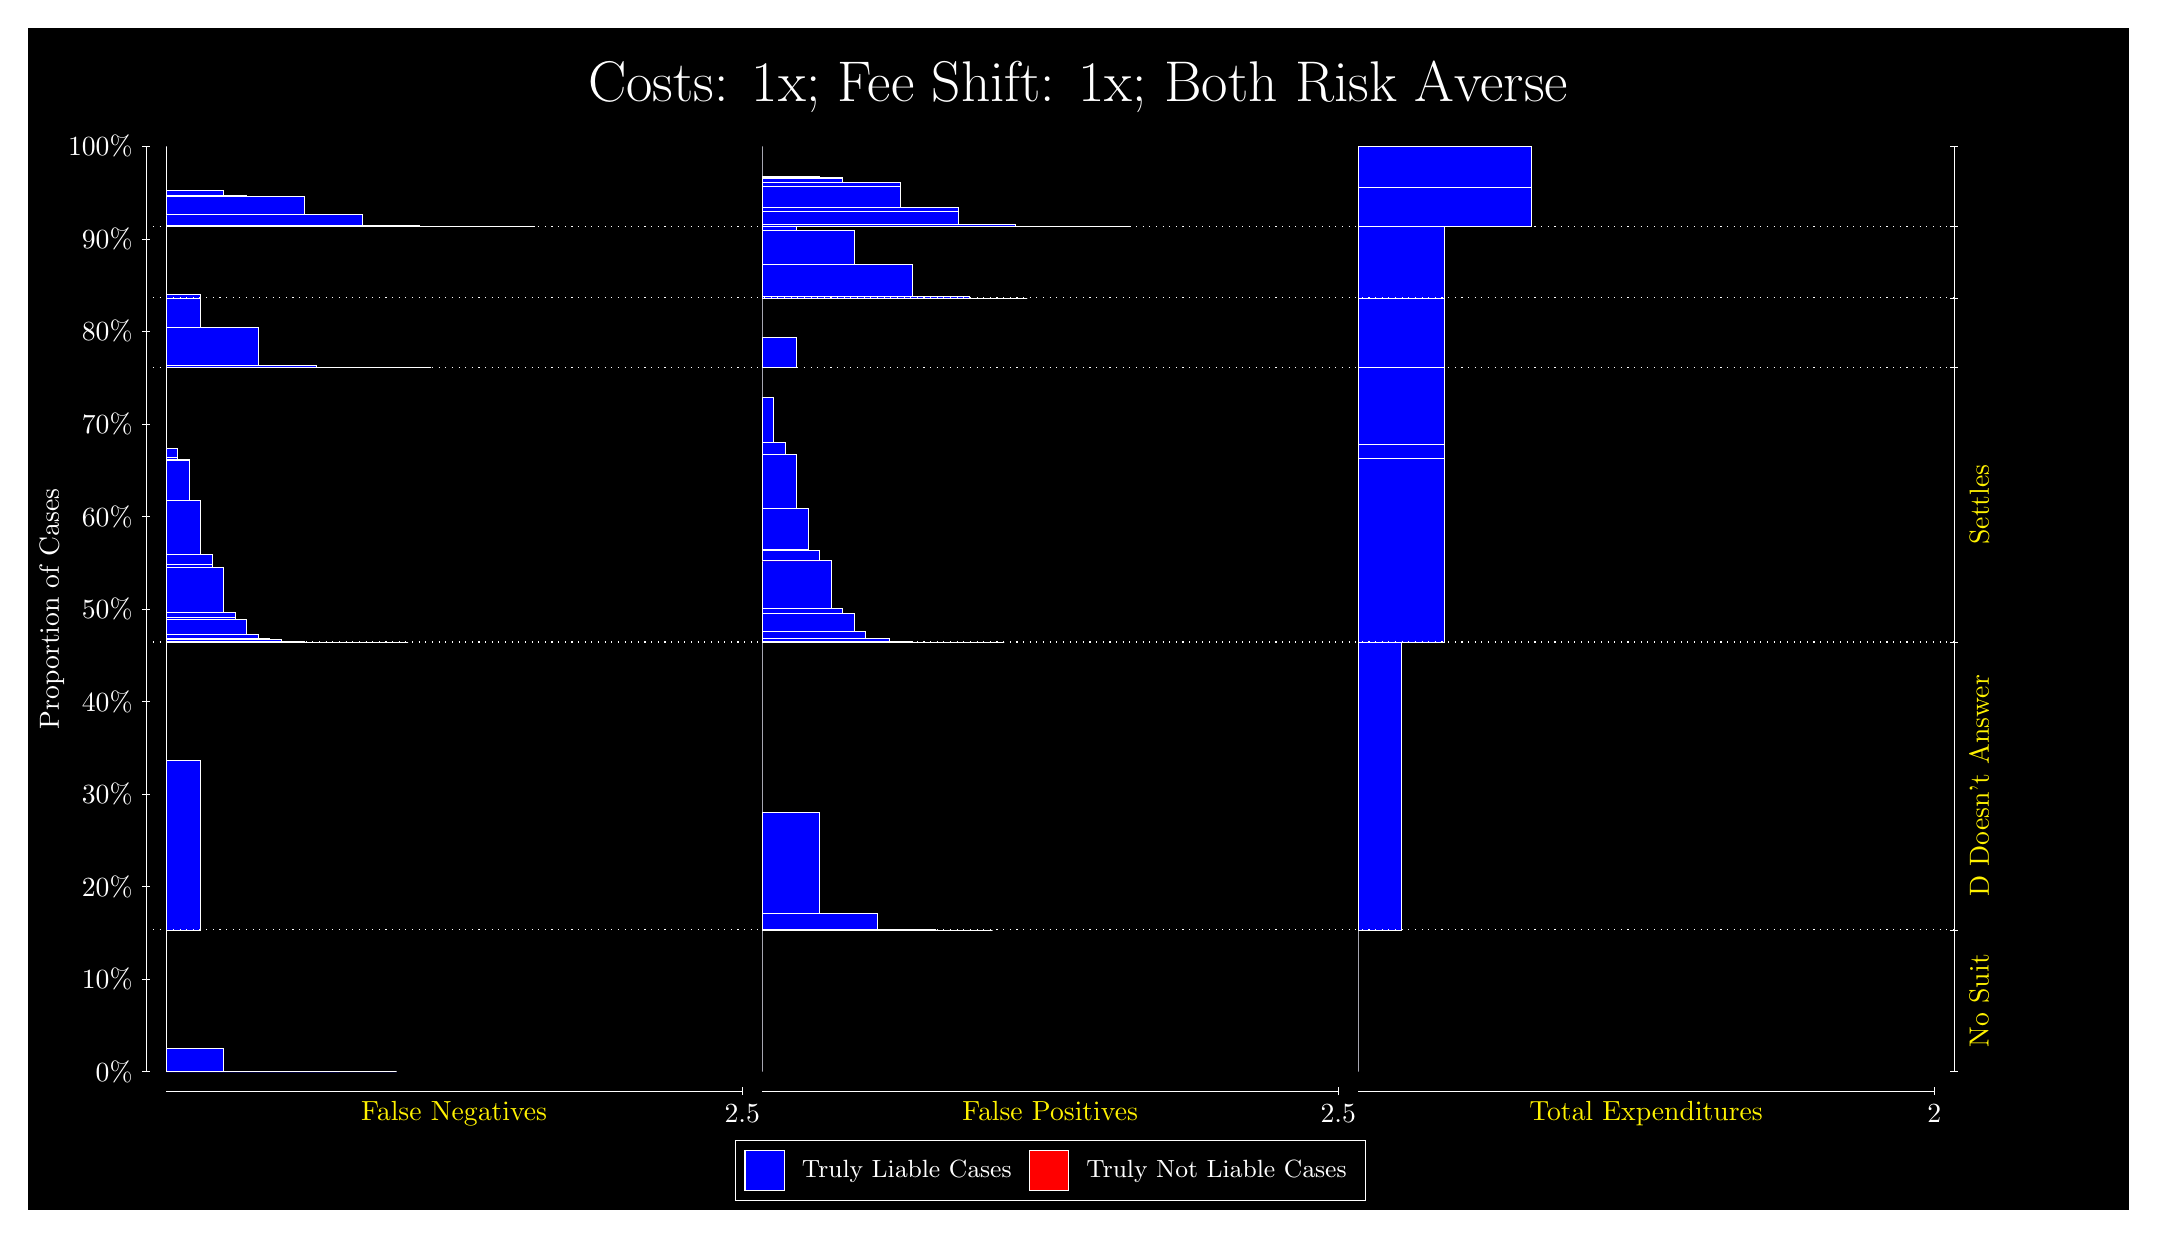
\begin{tikzpicture}
\draw[fill=black] (0,0) rectangle (26.667,15);
\draw[text=white] (0,13.5) rectangle (26.667,15) node[midway] {\huge Costs: 1x; Fee Shift: 1x; Both Risk Averse};
\draw[white, very thin] (1.5,1.75) -- (1.5,13.5);
\node[rotate=90, text=white, anchor=center] at (0.3, 7.625) {Proportion of Cases};
\draw[white, very thin] (1.45,1.75) -- (1.55,1.75);
\node[text=white, anchor=east] at (1.45, 1.75) {0\%};
\draw[white, very thin] (1.45,2.925) -- (1.55,2.925);
\node[text=white, anchor=east] at (1.45, 2.925) {10\%};
\draw[white, very thin] (1.45,4.1) -- (1.55,4.1);
\node[text=white, anchor=east] at (1.45, 4.1) {20\%};
\draw[white, very thin] (1.45,5.275) -- (1.55,5.275);
\node[text=white, anchor=east] at (1.45, 5.275) {30\%};
\draw[white, very thin] (1.45,6.45) -- (1.55,6.45);
\node[text=white, anchor=east] at (1.45, 6.45) {40\%};
\draw[white, very thin] (1.45,7.625) -- (1.55,7.625);
\node[text=white, anchor=east] at (1.45, 7.625) {50\%};
\draw[white, very thin] (1.45,8.8) -- (1.55,8.8);
\node[text=white, anchor=east] at (1.45, 8.8) {60\%};
\draw[white, very thin] (1.45,9.975) -- (1.55,9.975);
\node[text=white, anchor=east] at (1.45, 9.975) {70\%};
\draw[white, very thin] (1.45,11.15) -- (1.55,11.15);
\node[text=white, anchor=east] at (1.45, 11.15) {80\%};
\draw[white, very thin] (1.45,12.325) -- (1.55,12.325);
\node[text=white, anchor=east] at (1.45, 12.325) {90\%};
\draw[white, very thin] (1.45,13.5) -- (1.55,13.5);
\node[text=white, anchor=east] at (1.45, 13.5) {100\%};

\draw[white, very thin] (24.457,1.75) -- (24.457,13.5);
\draw[white, very thin] (24.407,1.75) -- (24.507,1.75);
\node[anchor=west] at (24.407, 1.75) {};
\draw[white, very thin] (24.407,3.5495) -- (24.507,3.5495);
\node[anchor=west] at (24.407, 3.5495) {};
\draw[white, very thin] (24.407,7.2047) -- (24.507,7.2047);
\node[anchor=west] at (24.407, 7.2047) {};
\draw[white, very thin] (24.407,10.695) -- (24.507,10.695);
\node[anchor=west] at (24.407, 10.695) {};
\draw[white, very thin] (24.407,11.575) -- (24.507,11.575);
\node[anchor=west] at (24.407, 11.575) {};
\draw[white, very thin] (24.407,12.487) -- (24.507,12.487);
\node[anchor=west] at (24.407, 12.487) {};
\draw[white, very thin] (24.407,13.5) -- (24.507,13.5);
\node[anchor=west] at (24.407, 13.5) {};

\draw[white, very thin, fill=blue] (1.75,1.75) rectangle (4.6775,1.75);
\draw[white, very thin, fill=blue] (1.75,1.75) rectangle (3.9457,1.75);
\draw[white, very thin, fill=blue] (1.75,1.75) rectangle (3.2138,1.7525);
\draw[white, very thin, fill=blue] (1.75,1.7525) rectangle (2.4819,2.0446);
\draw[white, very thin, fill=red] (1.75,2.0446) rectangle (1.75,2.0446);
\draw[white, very thin, fill=blue] (1.75,2.0446) rectangle (1.75,3.5495);
\draw[white, very thin, fill=blue] (1.75,3.5495) rectangle (2.1891,5.7061);
\draw[white, very thin, fill=red] (1.75,5.7061) rectangle (1.75,5.7061);
\draw[white, very thin, fill=blue] (1.75,5.7061) rectangle (1.75,7.2047);
\draw[white, very thin, fill=blue] (1.75,7.2047) rectangle (4.8239,7.2047);
\draw[white, very thin, fill=blue] (1.75,7.2047) rectangle (4.5312,7.2047);
\draw[white, very thin, fill=blue] (1.75,7.2047) rectangle (4.2384,7.2047);
\draw[white, very thin, fill=blue] (1.75,7.2047) rectangle (4.092,7.2047);
\draw[white, very thin, fill=blue] (1.75,7.2047) rectangle (3.9457,7.2047);
\draw[white, very thin, fill=blue] (1.75,7.2047) rectangle (3.7993,7.2048);
\draw[white, very thin, fill=blue] (1.75,7.2048) rectangle (3.6529,7.2048);
\draw[white, very thin, fill=blue] (1.75,7.2048) rectangle (3.5065,7.2141);
\draw[white, very thin, fill=blue] (1.75,7.2141) rectangle (3.3602,7.2162);
\draw[white, very thin, fill=blue] (1.75,7.2162) rectangle (3.2138,7.2404);
\draw[white, very thin, fill=blue] (1.75,7.2404) rectangle (3.0674,7.2406);
\draw[white, very thin, fill=blue] (1.75,7.2406) rectangle (3.0674,7.2539);
\draw[white, very thin, fill=blue] (1.75,7.2539) rectangle (2.921,7.2999);
\draw[white, very thin, fill=blue] (1.75,7.2999) rectangle (2.7746,7.4935);
\draw[white, very thin, fill=blue] (1.75,7.4935) rectangle (2.6283,7.5195);
\draw[white, very thin, fill=blue] (1.75,7.5195) rectangle (2.6283,7.5863);
\draw[white, very thin, fill=blue] (1.75,7.5863) rectangle (2.4819,8.1602);
\draw[white, very thin, fill=blue] (1.75,8.1602) rectangle (2.3355,8.1895);
\draw[white, very thin, fill=blue] (1.75,8.1895) rectangle (2.3355,8.3145);
\draw[white, very thin, fill=blue] (1.75,8.3145) rectangle (2.1891,9.0024);
\draw[white, very thin, fill=blue] (1.75,9.0024) rectangle (2.0428,9.5159);
\draw[white, very thin, fill=blue] (1.75,9.5159) rectangle (2.0428,9.5236);
\draw[white, very thin, fill=blue] (1.75,9.5236) rectangle (1.8964,9.5553);
\draw[white, very thin, fill=blue] (1.75,9.5553) rectangle (1.8964,9.6629);
\draw[white, very thin, fill=blue] (1.75,9.6629) rectangle (1.75,9.663);
\draw[white, very thin, fill=red] (1.75,9.663) rectangle (1.75,9.663);
\draw[white, very thin, fill=blue] (1.75,9.663) rectangle (1.75,10.695);
\draw[white, very thin, fill=blue] (1.75,10.695) rectangle (5.1167,10.695);
\draw[white, very thin, fill=blue] (1.75,10.695) rectangle (4.3848,10.695);
\draw[white, very thin, fill=blue] (1.75,10.695) rectangle (3.6529,10.725);
\draw[white, very thin, fill=blue] (1.75,10.725) rectangle (2.921,11.197);
\draw[white, very thin, fill=blue] (1.75,11.197) rectangle (2.1891,11.575);
\draw[white, very thin, fill=red] (1.75,11.575) rectangle (1.75,11.575);
\draw[white, very thin, fill=blue] (1.75,11.575) rectangle (2.1891,11.625);
\draw[white, very thin, fill=red] (1.75,11.625) rectangle (1.75,11.625);
\draw[white, very thin, fill=blue] (1.75,11.625) rectangle (1.75,12.487);
\draw[white, very thin, fill=blue] (1.75,12.487) rectangle (6.4341,12.487);
\draw[white, very thin, fill=blue] (1.75,12.487) rectangle (5.7022,12.487);
\draw[white, very thin, fill=blue] (1.75,12.487) rectangle (4.9703,12.498);
\draw[white, very thin, fill=blue] (1.75,12.498) rectangle (4.2384,12.633);
\draw[white, very thin, fill=blue] (1.75,12.633) rectangle (3.9457,12.633);
\draw[white, very thin, fill=blue] (1.75,12.633) rectangle (3.5065,12.865);
\draw[white, very thin, fill=blue] (1.75,12.865) rectangle (3.2138,12.867);
\draw[white, very thin, fill=blue] (1.75,12.867) rectangle (2.7746,12.882);
\draw[white, very thin, fill=blue] (1.75,12.882) rectangle (2.4819,12.942);
\draw[white, very thin, fill=blue] (1.75,12.942) rectangle (2.0428,12.942);
\draw[white, very thin, fill=red] (1.75,12.942) rectangle (1.75,12.942);
\draw[white, very thin, fill=blue] (1.75,12.942) rectangle (1.75,13.5);
\draw[white, very thin, fill=red] (9.3189,1.75) rectangle (9.3189,1.75);
\draw[white, very thin, fill=blue] (9.3189,1.75) rectangle (9.3189,3.5495);
\draw[white, very thin, fill=red] (9.3189,3.5495) rectangle (12.246,3.5495);
\draw[white, very thin, fill=blue] (9.3189,3.5495) rectangle (12.246,3.5495);
\draw[white, very thin, fill=blue] (9.3189,3.5495) rectangle (11.515,3.5511);
\draw[white, very thin, fill=blue] (9.3189,3.5511) rectangle (10.783,3.7642);
\draw[white, very thin, fill=blue] (9.3189,3.7642) rectangle (10.051,5.048);
\draw[white, very thin, fill=blue] (9.3189,5.048) rectangle (9.3189,7.2047);
\draw[white, very thin, fill=red] (9.3189,7.2047) rectangle (12.393,7.2047);
\draw[white, very thin, fill=blue] (9.3189,7.2047) rectangle (12.393,7.2047);
\draw[white, very thin, fill=red] (9.3189,7.2047) rectangle (12.1,7.2047);
\draw[white, very thin, fill=blue] (9.3189,7.2047) rectangle (12.1,7.2047);
\draw[white, very thin, fill=red] (9.3189,7.2047) rectangle (11.807,7.2047);
\draw[white, very thin, fill=blue] (9.3189,7.2047) rectangle (11.807,7.2047);
\draw[white, very thin, fill=blue] (9.3189,7.2047) rectangle (11.661,7.2047);
\draw[white, very thin, fill=red] (9.3189,7.2047) rectangle (11.515,7.2047);
\draw[white, very thin, fill=blue] (9.3189,7.2047) rectangle (11.515,7.2047);
\draw[white, very thin, fill=blue] (9.3189,7.2047) rectangle (11.368,7.2047);
\draw[white, very thin, fill=red] (9.3189,7.2047) rectangle (11.222,7.2047);
\draw[white, very thin, fill=blue] (9.3189,7.2047) rectangle (11.222,7.2167);
\draw[white, very thin, fill=blue] (9.3189,7.2167) rectangle (11.075,7.2168);
\draw[white, very thin, fill=red] (9.3189,7.2168) rectangle (10.929,7.2168);
\draw[white, very thin, fill=blue] (9.3189,7.2168) rectangle (10.929,7.2519);
\draw[white, very thin, fill=red] (9.3189,7.2519) rectangle (10.929,7.2519);
\draw[white, very thin, fill=blue] (9.3189,7.2519) rectangle (10.929,7.2519);
\draw[white, very thin, fill=blue] (9.3189,7.2519) rectangle (10.783,7.2521);
\draw[white, very thin, fill=blue] (9.3189,7.2521) rectangle (10.636,7.2536);
\draw[white, very thin, fill=red] (9.3189,7.2536) rectangle (10.636,7.2536);
\draw[white, very thin, fill=blue] (9.3189,7.2536) rectangle (10.636,7.3415);
\draw[white, very thin, fill=blue] (9.3189,7.3415) rectangle (10.49,7.5699);
\draw[white, very thin, fill=red] (9.3189,7.5699) rectangle (10.344,7.5699);
\draw[white, very thin, fill=blue] (9.3189,7.5699) rectangle (10.344,7.6332);
\draw[white, very thin, fill=blue] (9.3189,7.6332) rectangle (10.197,8.2367);
\draw[white, very thin, fill=blue] (9.3189,8.2367) rectangle (10.197,8.2368);
\draw[white, very thin, fill=red] (9.3189,8.2368) rectangle (10.051,8.2368);
\draw[white, very thin, fill=blue] (9.3189,8.2368) rectangle (10.051,8.3761);
\draw[white, very thin, fill=blue] (9.3189,8.3761) rectangle (9.9044,8.3838);
\draw[white, very thin, fill=blue] (9.3189,8.3838) rectangle (9.9044,8.8973);
\draw[white, very thin, fill=blue] (9.3189,8.8973) rectangle (9.758,9.5852);
\draw[white, very thin, fill=blue] (9.3189,9.5852) rectangle (9.6116,9.7395);
\draw[white, very thin, fill=blue] (9.3189,9.7395) rectangle (9.4652,10.313);
\draw[white, very thin, fill=blue] (9.3189,10.313) rectangle (9.4652,10.313);
\draw[white, very thin, fill=blue] (9.3189,10.313) rectangle (9.3189,10.695);
\draw[white, very thin, fill=red] (9.3189,10.695) rectangle (9.758,10.695);
\draw[white, very thin, fill=blue] (9.3189,10.695) rectangle (9.758,11.073);
\draw[white, very thin, fill=blue] (9.3189,11.073) rectangle (9.3189,11.575);
\draw[white, very thin, fill=red] (9.3189,11.575) rectangle (12.686,11.575);
\draw[white, very thin, fill=blue] (9.3189,11.575) rectangle (12.686,11.575);
\draw[white, very thin, fill=blue] (9.3189,11.575) rectangle (11.954,11.601);
\draw[white, very thin, fill=blue] (9.3189,11.601) rectangle (11.222,11.999);
\draw[white, very thin, fill=blue] (9.3189,11.999) rectangle (10.49,12.437);
\draw[white, very thin, fill=blue] (9.3189,12.437) rectangle (9.758,12.487);
\draw[white, very thin, fill=red] (9.3189,12.487) rectangle (14.003,12.487);
\draw[white, very thin, fill=blue] (9.3189,12.487) rectangle (14.003,12.487);
\draw[white, very thin, fill=red] (9.3189,12.487) rectangle (13.271,12.487);
\draw[white, very thin, fill=blue] (9.3189,12.487) rectangle (13.271,12.488);
\draw[white, very thin, fill=red] (9.3189,12.488) rectangle (12.539,12.488);
\draw[white, very thin, fill=blue] (9.3189,12.488) rectangle (12.539,12.504);
\draw[white, very thin, fill=blue] (9.3189,12.504) rectangle (11.807,12.674);
\draw[white, very thin, fill=red] (9.3189,12.674) rectangle (11.807,12.674);
\draw[white, very thin, fill=blue] (9.3189,12.674) rectangle (11.807,12.725);
\draw[white, very thin, fill=blue] (9.3189,12.725) rectangle (11.075,12.987);
\draw[white, very thin, fill=blue] (9.3189,12.987) rectangle (11.075,13.045);
\draw[white, very thin, fill=red] (9.3189,13.045) rectangle (10.783,13.045);
\draw[white, very thin, fill=blue] (9.3189,13.045) rectangle (10.783,13.045);
\draw[white, very thin, fill=blue] (9.3189,13.045) rectangle (10.344,13.093);
\draw[white, very thin, fill=blue] (9.3189,13.093) rectangle (10.344,13.105);
\draw[white, very thin, fill=red] (9.3189,13.105) rectangle (10.051,13.105);
\draw[white, very thin, fill=blue] (9.3189,13.105) rectangle (10.051,13.12);
\draw[white, very thin, fill=blue] (9.3189,13.12) rectangle (9.6116,13.121);
\draw[white, very thin, fill=blue] (9.3189,13.121) rectangle (9.6116,13.122);
\draw[white, very thin, fill=red] (9.3189,13.122) rectangle (9.3189,13.122);
\draw[white, very thin, fill=blue] (9.3189,13.122) rectangle (9.3189,13.5);
\draw[white, very thin, fill=red] (16.888,1.75) rectangle (16.888,1.75);
\draw[white, very thin, fill=blue] (16.888,1.75) rectangle (16.888,3.5495);
\draw[white, very thin, fill=red] (16.888,3.5495) rectangle (17.437,3.5495);
\draw[white, very thin, fill=blue] (16.888,3.5495) rectangle (17.437,7.2047);
\draw[white, very thin, fill=red] (16.888,7.2047) rectangle (17.986,7.2047);
\draw[white, very thin, fill=blue] (16.888,7.2047) rectangle (17.986,9.5417);
\draw[white, very thin, fill=red] (16.888,9.5417) rectangle (17.986,9.5417);
\draw[white, very thin, fill=blue] (16.888,9.5417) rectangle (17.986,9.7181);
\draw[white, very thin, fill=red] (16.888,9.7181) rectangle (17.986,9.7181);
\draw[white, very thin, fill=blue] (16.888,9.7181) rectangle (17.986,10.695);
\draw[white, very thin, fill=red] (16.888,10.695) rectangle (17.986,10.695);
\draw[white, very thin, fill=blue] (16.888,10.695) rectangle (17.986,11.575);
\draw[white, very thin, fill=red] (16.888,11.575) rectangle (17.986,11.575);
\draw[white, very thin, fill=blue] (16.888,11.575) rectangle (17.986,12.487);
\draw[white, very thin, fill=red] (16.888,12.487) rectangle (19.083,12.487);
\draw[white, very thin, fill=blue] (16.888,12.487) rectangle (19.083,12.985);
\draw[white, very thin, fill=red] (16.888,12.985) rectangle (19.083,12.985);
\draw[white, very thin, fill=blue] (16.888,12.985) rectangle (19.083,13.5);
\draw[white, dotted] (1.5,3.5495) -- (24.457,3.5495);
\draw[white, dotted] (1.5,7.2047) -- (24.457,7.2047);
\draw[white, dotted] (1.5,10.695) -- (24.457,10.695);
\draw[white, dotted] (1.5,11.575) -- (24.457,11.575);
\draw[white, dotted] (1.5,12.487) -- (24.457,12.487);
\draw[white, very thin] (1.75,1.5) -- (9.0689,1.5);
\node[text=yellow, anchor=north] at (5.4094, 1.5) {False Negatives};
\draw[white, very thin] (9.0689,1.45) -- (9.0689,1.55);
\node[text=white, anchor=north] at (9.0689, 1.45) {2.5};

\draw[white, very thin] (9.3189,1.5) -- (16.638,1.5);
\node[text=yellow, anchor=north] at (12.978, 1.5) {False Positives};
\draw[white, very thin] (16.638,1.45) -- (16.638,1.55);
\node[text=white, anchor=north] at (16.638, 1.45) {2.5};

\draw[white, very thin] (16.888,1.5) -- (24.207,1.5);
\node[text=yellow, anchor=north] at (20.547, 1.5) {Total Expenditures};
\draw[white, very thin] (24.207,1.45) -- (24.207,1.55);
\node[text=white, anchor=north] at (24.207, 1.45) {2};

\node[text=yellow, centered, rotate=90] at (24.777, 2.6497) {No Suit};
\node[text=yellow, centered, rotate=90] at (24.777, 5.3771) {D Doesn't Answer};
\node[text=yellow, centered, rotate=90] at (24.777, 8.9499) {Settles};




\draw (12.978300999999998,1.5) node[draw=none] (baseCoordinate) {};
\begin{scope}[align=center]
        \matrix[scale=0.5, draw=white, below=0.5cm of baseCoordinate, nodes={draw}, column sep=0.1cm]{
            \node[rectangle, draw, minimum width=0.5cm, minimum height=0.5cm, fill=blue] {}; &
            \node[draw=none, font=\small, text=white] (B) {Truly Liable Cases}; &
            \node[rectangle, draw, minimum width=0.5cm, minimum height=0.5cm, fill=red] {}; &
            \node[draw=none, font=\small, text=white] (B) {Truly Not Liable Cases}; \\
            };
\end{scope}

\end{tikzpicture}
\end{document}